\documentclass[a4j,12pt,]{jarticle}
 \usepackage{float}
 \usepackage{siunitx} %%SI単位系用
 \usepackage{amssymb, amsmath}
 \usepackage{ascmac,here,txfonts}
 \usepackage{hyperref}
 \usepackage{listings}
 \usepackage{pxjahyper}
 \usepackage[dvipdfmx]{graphicx}
 \usepackage{amssymb, amsmath}
  \usepackage{listings}
  \usepackage[dvipdfmx]{color}
 
 \lstset{
   language={Python},
   basicstyle={\ttfamily},
   identifierstyle={\small},
   commentstyle={\small\itshape},
   keywordstyle={\small\bfseries},
   ndkeywordstyle={\small},
   stringstyle={\small\ttfamily},
   frame={single},
   breaklines=true,
   columns=[l]{fullflexible},
   numbers=left,
   xrightmargin=0zw,
   xleftmargin=3zw,
   numberstyle={\scriptsize},
   stepnumber=1,
   numbersep=1zw,
   lineskip=-0.5ex,
 }
\begin{document}

{\noindent\small  \hfill\today}
\begin{center}
  {\Large 実測値と理論値の時刻合わせに関する報告}
\end{center}
\begin{flushright}
  祖父江匠真 \\
\end{flushright}

\section{概要}
本研究室によって小学校などに設置されている太陽発電計測システムの中で、まつやまRe・再来館に設置されているものを除くと、ほとんどがインターネットに接続されていないオフライン環境で計測が行われている。このため、パーソナルコンピュータの内部時計が経過時間とともにずれる現象が生じ、実測データのタイムスタンプが不正確になっている。

一方、まつやまRe・再来館に設置されている計測システムはインターネットに接続されたオンライン環境で運用されており、さらにシステムを実行しているラズベリーパイが24時間ごとに再起動されているため、内部時計は常に同期され、計測データのタイムスタンプも正確である。

そこで、まつやまRe・再来館で得られた実測データを対象に、実測データと太陽光発電シミュレーターにより生成された理論データのペアに対して、相互相関関数を用いた時刻合わせプログラムの実装が行われている。

まつやまRe・再来館の実測データはタイムスタンプのずれがないため、時刻合わせプログラムにこのデータを入力し、推定結果が0秒となることで、正しく動作していると判断できる。そのため、推定結果0秒を目標として実装が進められている。

現時点の進捗では、晴天時の1日分の実測データを用いて時刻合わせプログラムを実行した結果、アルゴリズムによっては50〜200秒程度のタイムスタンプのずれが生じており、さらなる改善が必要である。

\section{相互相関とは}
相互相関は、2つの信号の類似性を測定するために用いられる統計的手法である。具体的には、2つの信号の類似度を示す数値を算出し、信号間の関係を調査することができる。この数値が高ければ高いほど、2つの信号は互いに類似していると言える。相互相関は、信号処理や時系列データ解析において、信号の遅延やズレを検出する目的で幅広く活用されている。

相互相関を用いた信号間のズレの検出方法は以下の手順で行われる。

\begin{enumerate}
\item 2つの信号(信号Aおよび信号Bとする)を用意する。これらの信号は同じ長さであることが望ましいが、異なる場合でも適用が可能である。
\item 信号Aと信号Bをずらしながら重ね合わせる。このずらしの大きさを「ラグ」と称する。ラグが0である場合、信号Aと信号Bは完全に一致する状態である。ラグが正である場合、信号Bは信号Aより遅れていることを示し、ラグが負である場合はその逆である。
\item それぞれのラグにおいて、信号Aと信号Bの重ね合わせた部分の積の和(内積)を算出する。これを相互相関関数と呼ぶ。
\item それぞれのラグごとに相互相関関数を計算し、相互相関関数が最大となる際のラグを特定する。この際に得られたラグは、信号Aと信号Bのズレ時間を示している。
\end{enumerate}

例示すると、以下に示す2つの信号に対して相互相関を計算した場合、緑色の波形を右に800秒スライドさせた際に相互相関が最大となるため、これらの信号間のズレ時間は相互相関により800秒であると推定される。

\begin{figure}[H]
  \begin{center}
    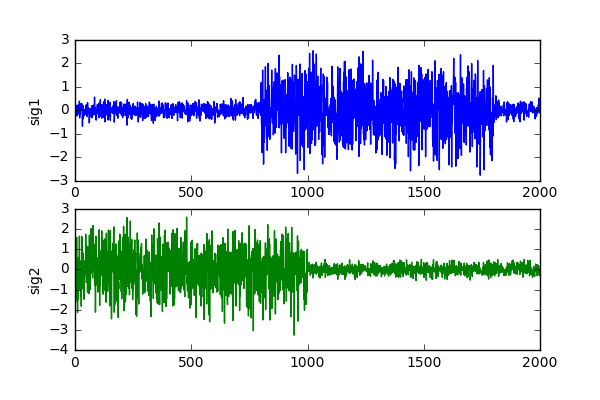
\includegraphics[width=160mm]{1.png}
    \caption{相互相関によるズレ時間の推定例}
    \label{p1}
  \end{center}
\end{figure}

相互相関を用いたズレの検出は、ノイズの影響を受けにくく、信号のパターンが不明な場合や信号の形状が複雑な場合でも、信号間の関係を正確に評価することが可能である。ただし、計算コストが高いため、大規模なデータやリアルタイムの信号処理においては、効率的なアルゴリズムや近似手法の検討が必要となる。相互相関は、信号解析や時系列データの処理において、多くのアプリケーションで有益な手法であり、その活用によって信号間の関係性の把握や信号の特性解析が行われている。今後も、さらなる研究開発によって、相互相関を用いた信号処理技術の向上が期待される。

\section{Pvlibを使用した理論データのシミュレーションについて}
Pvlibは、Pythonで実装された太陽光発電システムのシミュレーションを行うためのライブラリである。晴天の日における日射量の推定は、以下の手順で進める。

\begin{enumerate}
\item \textbf{位置情報の設定}: まず、緯度、経度、標高、タイムゾーンなどを指定し、\texttt{pvlib.location.Location}オブジェクトを生成する。このオブジェクトは、太陽位置や日射量の計算に使用される。
\item \textbf{日時データの準備}: 推定対象の日時範囲を指定し、対応する表データを作成する。
\item \textbf{太陽位置の計算}: \texttt{pvlib.solarposition.get\_solarposition}関数を用いて、指定された位置情報および日時データを基に、太陽の高度角と方位角を計算する。
\item \textbf{大気透過率の計算}: \texttt{pvlib.clearsky.ineichen}関数を使用し、大気透過率を計算する。この関数は、指定された位置情報と太陽位置に基づいて、大気の透過率を推定し、全天日射量、直達日射量、拡散日射量を計算する。
\item \textbf{地表での日射量の推定}: 最後に、\texttt{pvlib.irradiance.get\_total\_irradiance}関数を用いて、地表での日射量を推定する。この関数は、太陽位置、大気透過率、入射角などの情報に基づいて、地表での直達日射量、拡散日射量、反射日射量を計算する。
\end{enumerate}

これらの手順に従って、晴天の日における地表での日射量を推定することができる。得られた日射量データは、実測データとの比較に利用される。

例示すると、以下に示されているのは2022年4月8日に松山Re・再来館で計測された実測データである。

\begin{figure}[H]
  \begin{center}
    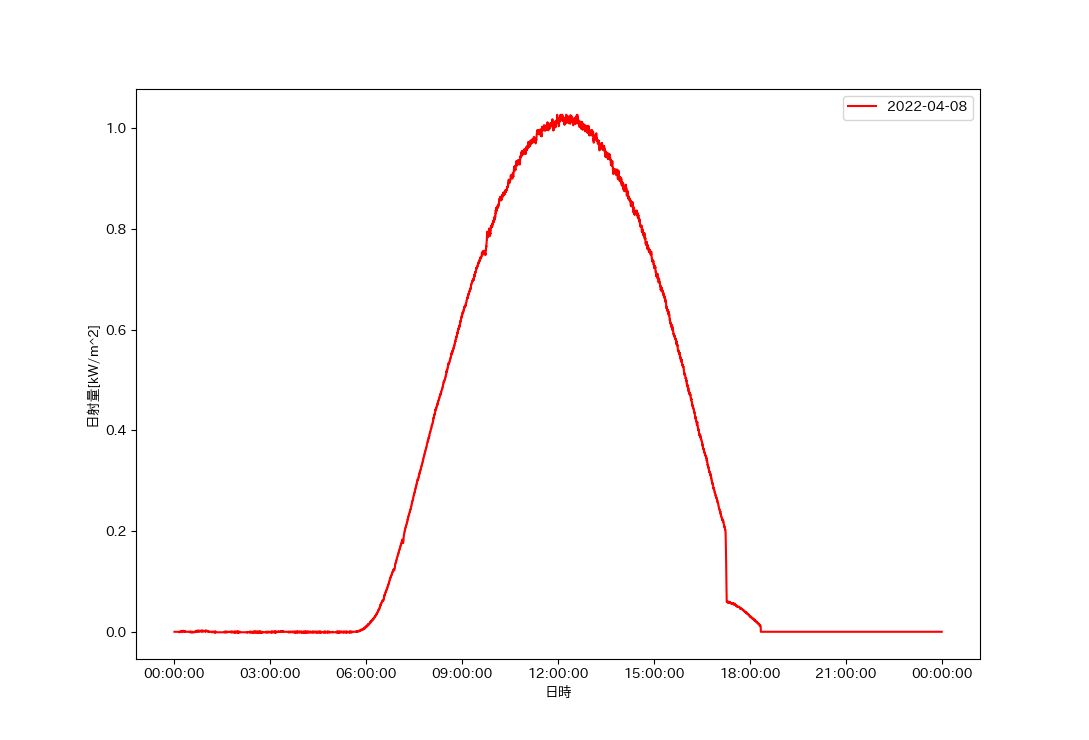
\includegraphics[width=160mm]{2.png}
    \caption{実測データ}
    \label{p2}
  \end{center}
\end{figure}

この実測データのタイムスタンプ列をPvlibに入力し、晴天の日におけるシミュレーション結果を以下に示す。

\begin{figure}[H]
  \begin{center}
    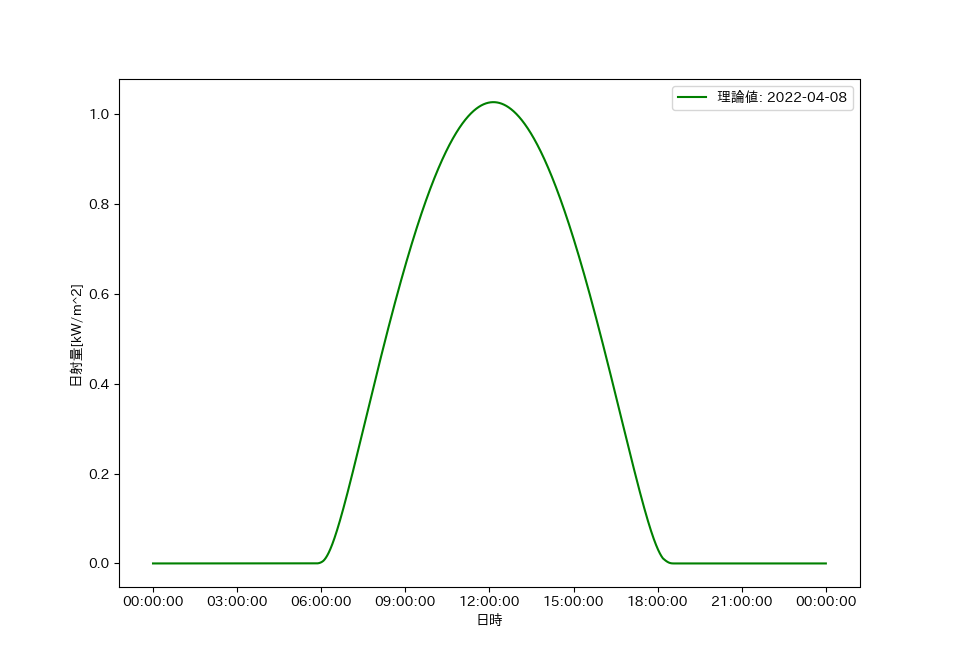
\includegraphics[width=160mm]{3.png}
    \caption{シミュレーション結果}
    \label{p3}
  \end{center}
\end{figure}

実測データと理論データを合わせてプロットする。

\begin{figure}[H]
  \begin{center}
    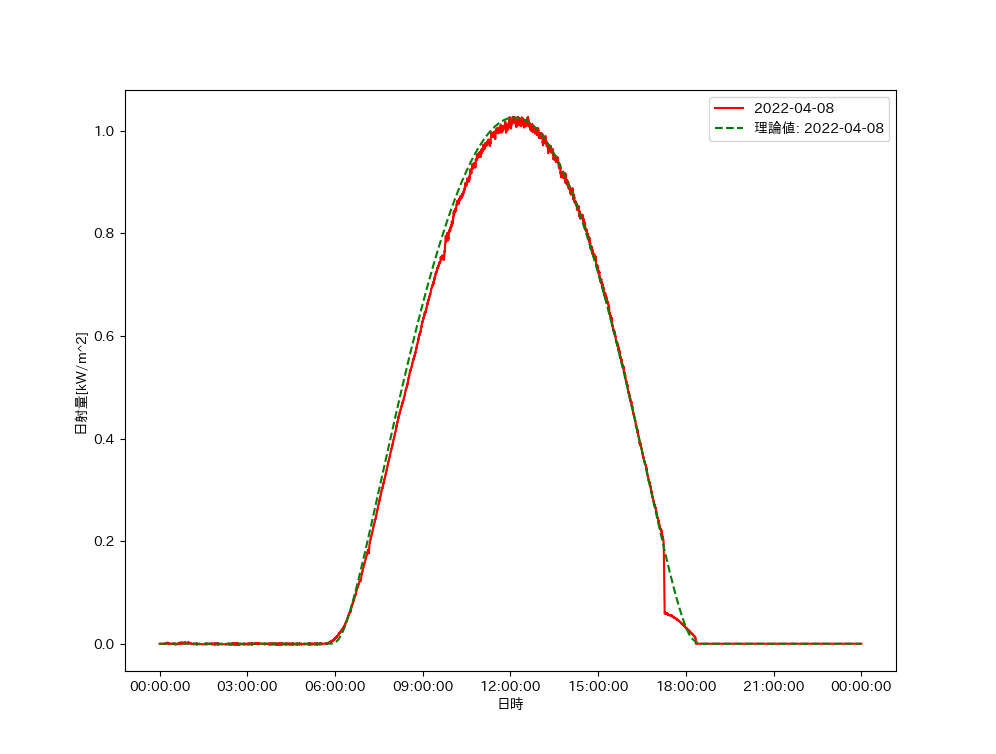
\includegraphics[width=160mm]{4.png}
    \caption{実測データと理論データのプロット}
    \label{p4}
  \end{center}
\end{figure}

このように晴天の日の実測データであれば、理論データは概ね一致する。

\section{時刻合わせプログラムの実装に関する検討}
現在実装されている時刻合わせプログラムでは、以下の手順で実測データと理論データのズレ時間を推定している。

\begin{enumerate}
\item まず実測データを読み込み、データのサンプリング間隔を1秒ごとの等間隔になるようリサンプリングするなど、前処理を実施する。
\item 次に実測データのタイムスタンプ情報を太陽光発電シミュレーターであるPvlibに入力し、晴天の日における松山Re・再来館の日射量を予測する。
\item 最後に、これらの実測データと理論データを用いて相互相関関数を計算し、最大相関値を持つインデックスを特定する。このインデックスが二つのデータのズレ時間を示し、インデックスに対応するラグがズレ時間となる。
\end{enumerate}

例えば、2022年4月8日の実測データに対してズレ時間を計算した結果、理論データに対して実測データを165秒進めたときに相互相関が最大となり、ズレ時間の推定結果は165秒となった。

\begin{figure}[H]
  \begin{center}
    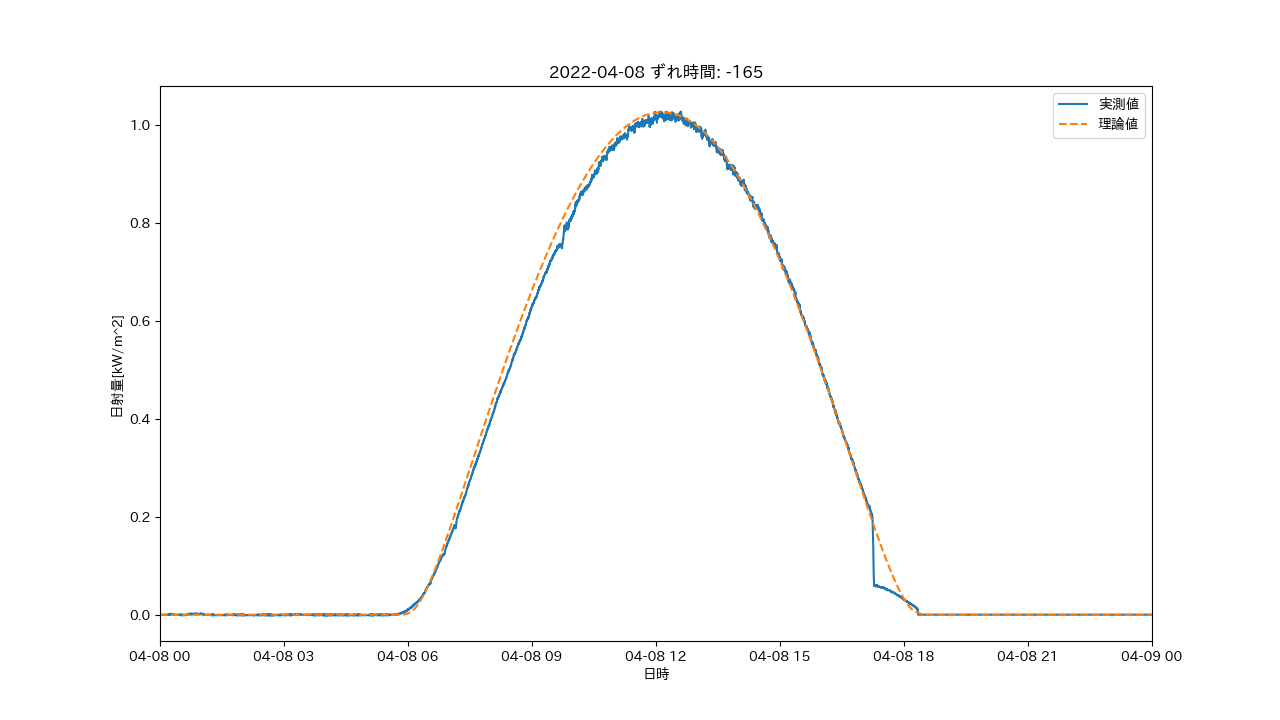
\includegraphics[width=160mm]{5.png}
    \caption{2022年4月8日の実測データと理論データの相互相関}
    \label{p5}
  \end{center}
\end{figure}

前処理では、実測データのリサンプリングの他に、実測データのフィルタリングや正規化などが行われる。この前処理の組み合わせ方によって相互相関によるズレ時間の推定結果が変化するため、様々な前処理の組み合わせを試みており、それぞれの組み合わせにおける相互相関の推定結果について検討する。

\subsection{指定期間外の日射量を0に置き換える実測データの前処理}
2022年4月8日の実測データを観察すると、日没前に日射量が急激に低下する箇所が存在する。

これは、おそらく松山Re・再来館の周辺にあるマンション等の建物によって太陽光が遮られることが原因と考えられる。このような実測データと理論データで日射量が大きく異なる箇所が相互相関の推定結果に影響を与えていると推測し、そのような箇所を実測データから除去する前処理を実施した。

以下に示す図は、2022年4月8日の実測データと理論データの日射量が大きく異ならない期間に限定してフィルタリングを行い、相互相関を計算したものである。

このフィルタリングでは、指定期間外の実測データと理論データの日射量を0に置き換えている。

\begin{figure}[H]
  \begin{center}
    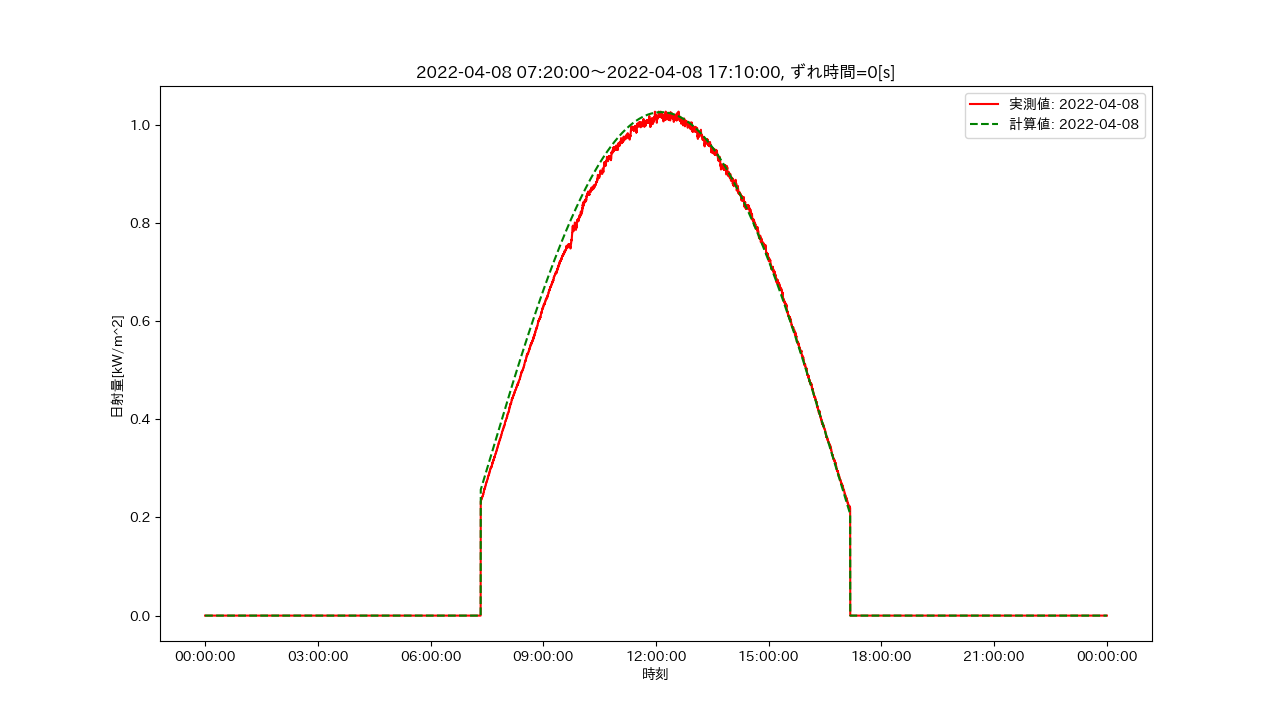
\includegraphics[width=160mm]{6.png}
    \caption{フィルタリング後の2022年4月8日の実測データと理論データの相互相関}
    \label{p6}
  \end{center}
\end{figure}

相互相関によるズレ時間の推定結果は0秒となり、一見うまくズレ時間を予測できているように見えるが、次の図に示すような理論データと大きく概形が異なる実測データとの相互相関でも同様にズレ時間の推定結果が0秒となってしまった。

\begin{figure}[H]
  \begin{center}
    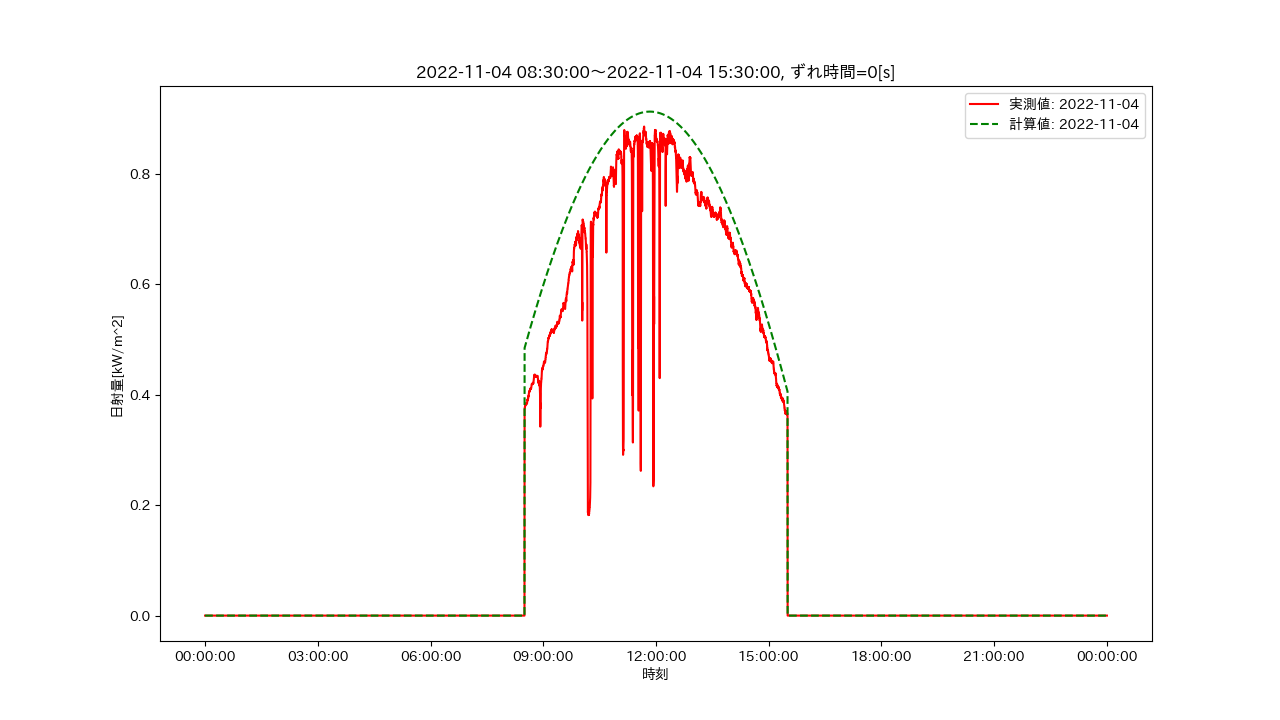
\includegraphics[width=160mm]{7.png}
    \caption{概形が異なる実測データと理論データの相互相関}
    \label{p7}
  \end{center}
\end{figure}

実測データの概形に関係なく、推定結果が常に0秒となってしまう原因としては、フィルタリング時に指定期間外の日射量を全て0に置き換えたことで、実測データと理論データの両方において指定期間の両端で日射量が0に急激に低下する箇所が現れ、この箇所が相互相関の計算時に強く作用することで、指定期間内の概形に関わらず、ズレ時間の推定結果が常に0秒になってしまうと考えられる。

\subsection{実測データに対する特定の日射量によるフィルタリングおよび日射量の減算}
「実測データを、指定した期間外の日射量が0になるように置き換える」という方法では、指定期間の両端において日射量が0に急激に低下する箇所が相互相関計算に強く影響し、その結果、相互相関による推定結果が常に0秒になると推測された。

従って、日射量が0へ急激に低下する箇所を作らない手法として、以下の図に示すように実測データの日射量を特定の値以下に切り落とすフィルタリングを行い、さらに指定した値だけ実測データを下方向にスライドさせる方法を採用した。

以下に示すのは2022/04/08の実測データと理論データであるが、この実測データを次の図に示すように日射量が0.2$\mathrm{kW}/\mathrm{m}^2$以上のみになるようフィルタリングする

\begin{figure}[H]
  \begin{center}
    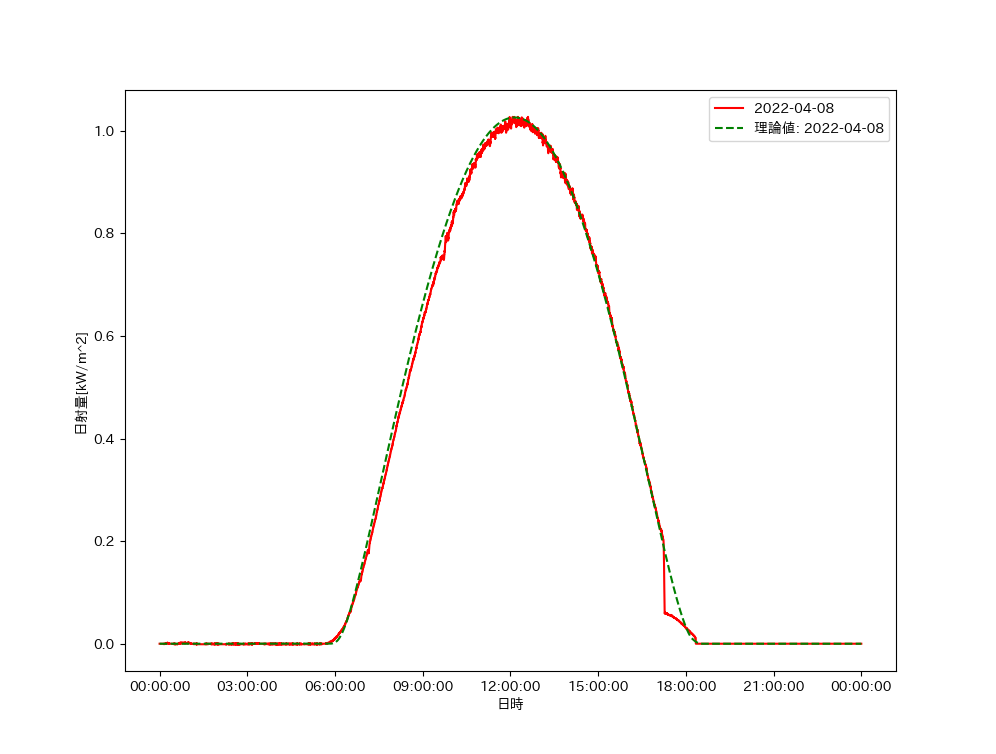
\includegraphics[width=160mm]{8.png}
    \caption{フィルタリング前の2022年4月8日の実測データ}
    \label{p8}
  \end{center}
\end{figure}

\begin{figure}[H]
  \begin{center}
    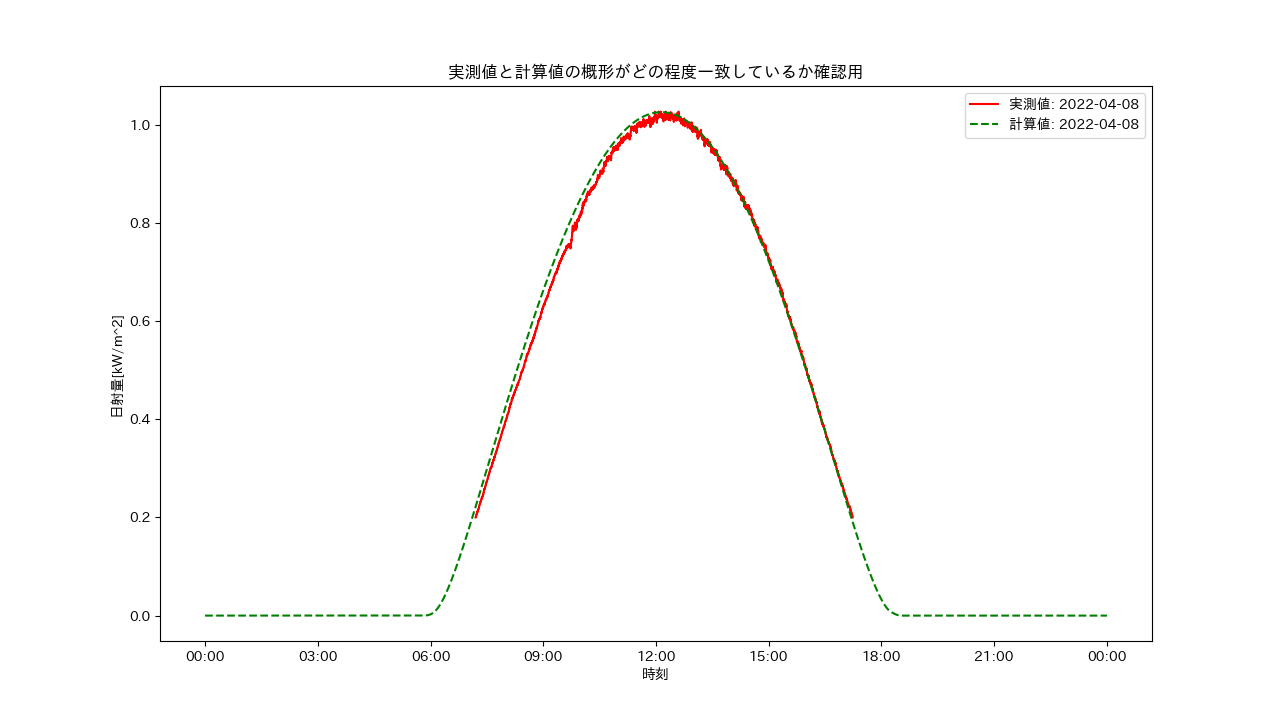
\includegraphics[width=160mm]{9.png}
    \caption{日射量が0.2$\mathrm{kW}/\mathrm{m}^2$以上のみになるようフィルタリングした実測データ}
    \label{p9}
  \end{center}
\end{figure}

そして、上の図の実測データから0.2を減算し、以下の図のようにする

\begin{figure}[H]
  \begin{center}
    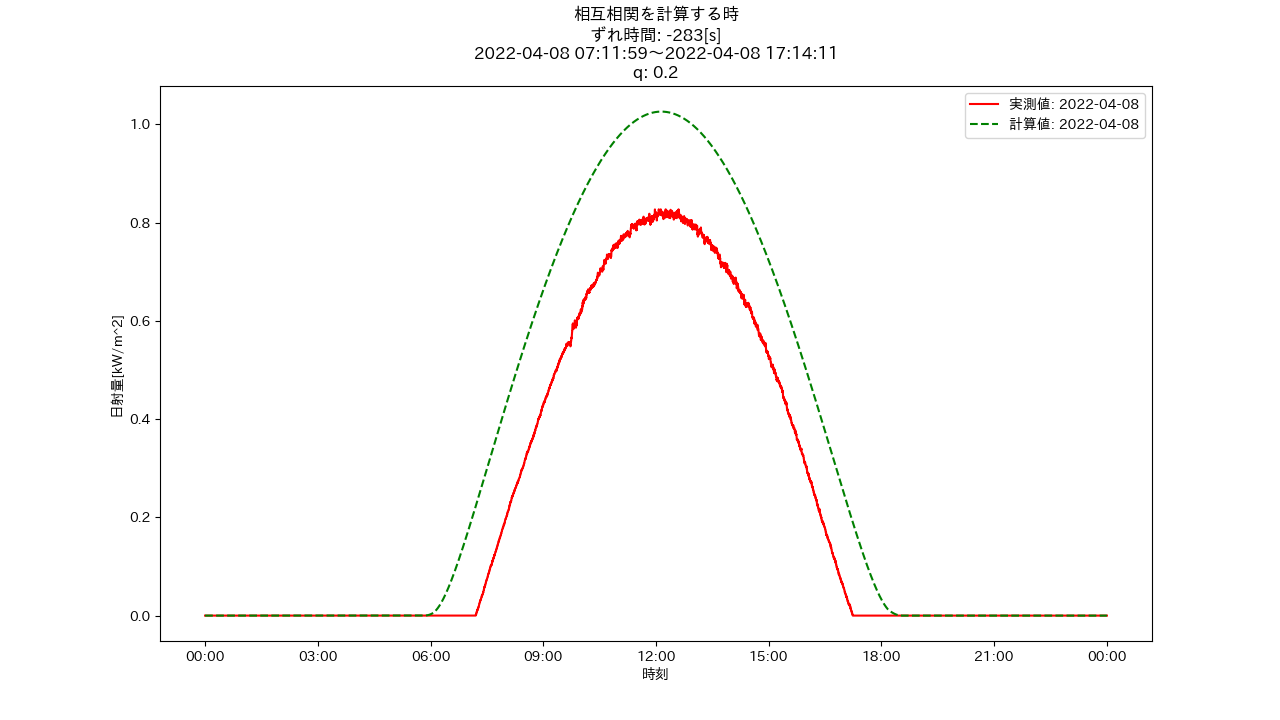
\includegraphics[width=160mm]{10.png}
    \caption{減算後の実測データ}
    \label{p10}
  \end{center}
\end{figure}

この方法により、フィルタリングの両端で相互相関計算に強く影響することによって、推定結果のズレ時間が常に0秒になる問題を回避できることが期待される。

しかしながら、2022年4月8日のデータにおいては、相互相関によるズレ時間の推定結果が-283秒となり、本前処理手法によってズレ時間の推定結果が改善されることは確認できなかった。

\section{まとめ}
晴天時における1日分の実測データを用いた場合、推定されたズレ時間は、真の値である0秒から平均して50〜200秒程度ずれていることが明らかとなった。この結果から、データの前処理方法や日射量シミュレーションアルゴリズムの改良が必要であることが示唆されている。

具体的には、高精度な相関計算手法の導入や、データ前処理手法の改善が検討されるべきである。さらに、異なる日や天候条件下における実測データを用いて、プログラムの汎用性を評価することも重要であると考えられる。

\end{document}